\chapter{Methodology}
\label{Method}

\section{Mode I fracture loading test using the MMCG specimen: data reduction}

\section{Python Code to analysed datas}

\begin{lstlisting}[language=Python]
import numpy as np

def incmatrix(genl1,genl2):
    m = len(genl1)
    n = len(genl2)
    M = None #to become the incidence matrix
    VT = np.zeros((n*m,1), int)  #dummy variable

    #compute the bitwise xor matrix
    M1 = bitxormatrix(genl1)
    M2 = np.triu(bitxormatrix(genl2),1)

    for i in range(m-1):
        for j in range(i+1, m):
            [r,c] = np.where(M2 == M1[i,j])
            for k in range(len(r)):
                VT[(i)*n + r[k]] = 1;
                VT[(i)*n + c[k]] = 1;
                VT[(j)*n + r[k]] = 1;
                VT[(j)*n + c[k]] = 1;

                if M is None:
                    M = np.copy(VT)
                else:
                    M = np.concatenate((M, VT), 1)

                VT = np.zeros((n*m,1), int)

    return M
\end{lstlisting}

\lstinputlisting[language=Python, firstline=180, lastline=202]{Codes/pyMMCG.py}

The Python code developed is inspired from a previous one, done in MatLab by \parencite{Reference14} for DCB tests. MMCG specimen was created from DCB one, so it was logical to use this program with an adaptation to Python tools. A first program, allows to combine all the constants by creating a structure as :

\begin{customFrame}
# pixel to mm magnification factor
Test.mm2pixel = LX / H
# Load conversion factor - testing machine
Test.LoadConvFactor = 50  # N/V (gain = 500 N)
# Displacement conversion factor - testing machine
Test.DisplConvFactor = 2.0  # mm/V (gain = 20 mm)
Test.thickness = 12.5 # unit  mm
Test.a0 = 20 # unit  mm
###################################################
# Summary of DIC Settings
MatchID.CorrelationCoef = 'ZNSSD'
MatchID.InterpolationOrder = 'Bicubic spline'
MatchID.TransformationOrder = 'Affine'
MatchID.Subset, MatchID.Step = 15, 13
# Summary of Strain Settings
MatchID.StrainWindow = 5
MatchID.StrainConvention = 'GreenLagrange'
MatchID.StrainInterpolation = 'Q4'
# Area of Interest
MatchID.Roi_PolyXi, MatchID.Roi_PolyYi = 52, 259
MatchID.Roi_PolyXf, MatchID.Roi_PolyYf = 1587, 1119
###################################################
# Selecting subset directly from MatdhID
a0.imgH, a0.imgV = 1529, 669
# Selecting pair
COD.cod_pair = 2

\end{customFrame}

Thanks to this database file, open in the main code file, many calls can be done and allow to synthesize the main code. Of course one database was created for each specimen, due to the difference between values as the precrack length.
This main code is composed of several parts. First, after defining modules, path and opening all the necessary files as displacement csv file or strain one, it is important to read all the images from a single test. Indeed, it allows to know the number of stages (images) which must be run to obtain the entire test. Each stage gives a displacement of pixels, so un displacement of subsets, allowing to follow the crack length and the crack opening. It is important to note that MatchID allows to focus on a Zone of Interest (ZOI) in order to limit the amount of subsets read. According to \parencite{Reference7} dimensions of this ZOI are given for biggest specimens. By using equivalent dimensions, the ZOI adapted to this thesis is around 5,6cm length from the upper holes of the specimen and 2,8cm of width.

Then, by using the displacement depending on the axis, x and y, two folders are read, one with x displacements, the other with y displacements. In each folder, one test is composed of a number of files equal to the number of stages. It gives information about pixel movement. By reading these two folders, a first graphic is created, giving a representation of the specimen, with the subsets presented and the subset chosen to be the $a_{0}$ one (closer to the crack tip).

Then, a second part has the purpose to calculate the Crack Tip Opening Displacement (CTOD). MatchID is a great tool which does some work for the user. That is why, by using “wI aramis2D.csv” CTOD is almost find, depending on the time and the load applied. It is important to understand how it works. First, a part of the work is to define the zone of interest, the one where the crack must develop. It is done on MatchID, but also on Python by using the number of the subset defined by Match ID. Then, when a subset is out of this region, it will be considered as equal to zero. Then, the subset which are placed into the crack, or somewhere there is a default or missing information as into the crack, it will be decided to give this substep a value of -1. Then, for all the substep around the crack, which have a real interest in the study, they will take the value equal to 1. By using this matrix of substep, now, composed of -1, 0, 1 value, it is possible to plot the entire matrix into grey nuances, and have a look at the crack development, by adding matrix, given by different stages.

\begin{customFrame}
ud_lim = 10
# Uup, Udown, ||Uup-Udown||
CTODI  = np.zeros((ud_lim, 3, MatchID.stages))

for J in np.arange(0, MatchID.stages, 1):
# mode I:
uYtemp = np.copy(UY[:, :, J])
CTODI[:, 0, J] = np.flipud(uYtemp[a0.Y - ud_lim: a0.Y, a0.X])
CTODI[:, 1, J] = uYtemp[a0.Y: a0.Y + ud_lim, a0.X]
CTODI[:, 2, J] = np.abs(CTODI[:, 1, J] - CTODI[:, 0, J])
COD.wI = CTODI[COD.cod_pair, 2, :]
\end{customFrame}

To obtain CTOD, it is important to be careful to $a_{0}$ choice. Indeed, the chosen subset, will be determinant. Considering the image as a matrix composed of subset, the chosen subset as a position given by his m row and n column. To determinate the opening, it is necessary to have a look on the subsets in the same n column but at a different line. Indeed, the chosen subset will be the first one affected by the crack, that means, that information of the subset will not have importance anymore. While, looking to subset up and down allow to follow the displacement of the crack tip and measure it. The fact is to determine which pair of subsets is the best. The ones at the row n-1 and n+1, but maybe these ones will be on the crack at a given stage and we will lose all the necessary information. That is why, an important choice. Here COD pair was fixed equal to two.  Finally, by looking to the displacement of the pair of subsets, it is possible to obtain the value of the crack opening.

At least, a final step in this code is the determination of $a_{DIC}$. This parameter is the crack length, which evolves with time during all the experiment. This factor is the most difficult to obtain, indeed tools as MatchID cannot help the user to obtain the result stage by stage. The value of a(t) will be equal to $a_{0}$ fixed by the user and additional to a $\Delta a$ which is the value of the crack length, evolving in time due to the applied force.
\begin{customFrame}
roi = 'crop' # 'all'; 'crop'
i, incr = 1, 1
# incr : is used to step over stages if required (default = 1: all stages)
Y_i, Y_f = 0, UY.shape[0]
X_i, X_f = 0, a0.X
\end{customFrame}
To begin with, it is important to determinate a parameter, that we had called $\alpha$. This one is used on matrix as the M matrix. Indeed, M matrix represents, for a given stage, the crack length by having bigger value in the crack area as shown on \ref{fig:Fig11} :

\begin{figure}[h]
\centering
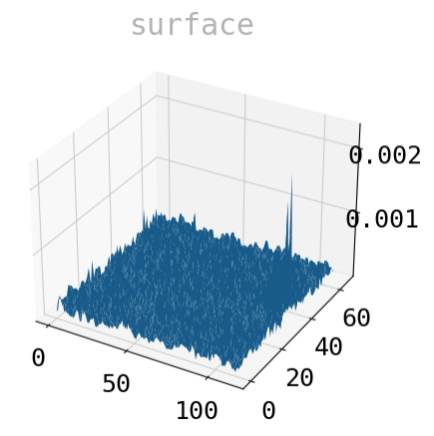
\includegraphics[scale=0.5]{Figures/M_matrix}
\decoRule
\caption[M matrix]{M matrix, obtained by running python code}
\label{fig:Fig11}
\end{figure}

As it is visible, if the user is looking too close, the noise of the values will avoid a good analyze, but by looking too high on the matrix, the crack length value will not be accurate. To move and have a precise idea of the way the user can watch the M matrix, it is important to use $\alpha$. Alpha parameter is like a cutting tool which allow to be as close as the noise without troubles.
To approximate the $\alpha$ value, a correlation factor is searched by least square regression method. The objective it to have the best linear part.
\begin{customFrame}
#### alpha evaluation :::::::::::::::::::::::::::::::::::::::::::::::::::::
### Selecting stage for investigating alpha
####

# least-squares linear regression
porder = 1
xx = Test.disp # displacement (mm)
yy = Test.load # load (N)
# Data point in the linear least-squares regression
limsup = int(0.75*np.argwhere(max(yy)==yy)[-1])
# number of maximum data points for LSR
liminf = int(np.round((1/3)*limsup))# number of minimum data points for LSR

xx, yy = xx[0:limsup], yy[0:limsup]
Rtot = np.zeros((limsup-liminf,1))
C_M = np.zeros((limsup-liminf,1))
for j in np.arange(0,limsup-liminf,1):
limt_sup = liminf + j
xfit, yfit = xx[0:limt_sup], yy[0:limt_sup]
p  = np.polyfit(xfit, yfit, porder)
C_M[j] = 1/p[0]
dev = yfit - np.mean(yfit) # deviations - measure of spread
SST = np.sum(dev**2) # total variation to be accounted for
resid = yfit - np.polyval(p, xfit) # residuals - measure of mismatch
SSE = np.sum(resid**2) # variation NOT accounted for
Rtot[j] = 1 - SSE/SST #  variation NOT accounted for

# position for the best fitting point parameters
jmax = np.max(np.argwhere(np.max(Rtot)==Rtot))
J = int(liminf + jmax)

### 2 criterion for checking stage
####
inb = 3
# standard deviation * inb (to be checked by user)
# inb = 1: 68.3 %
# inb = 2: 95.4 %
# inb = 3: 99.7 %
JJ = 1
while JJ == 1:
\end{customFrame}

\begin{figure}[h]
\centering
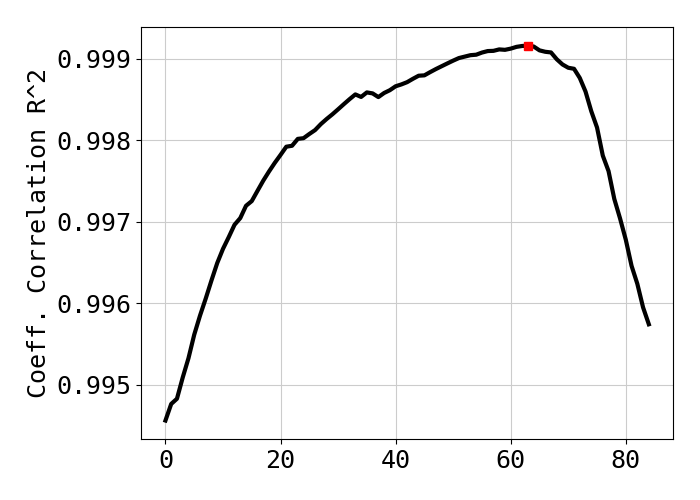
\includegraphics[scale=0.3]{Figures/Correlation_factor}
\decoRule
\caption[R correlation factor]{R correlation factor allowing to know which load and disalcement is linked to crack beggining.}
\label{fig:Fig12}
\end{figure}

The red dot shown on \ref{fig:Fig12}, is linked to another plot,

Then a matrix representing the subsets in the Area of Interest will be created. First this matrix is composed of zero. Then, the four corners of the matrix will be used to proceed several operations on the matrix. The external lines and columns will take a value of 2 and the corners a value of 4. The distance between opposite corners is calculated and their displacements are compared. Calling K, the maximal displacement of the two corners, average K and maximum one between all the steps are compared. Again, every subset is treated and are still zero when the material is undamaged. It becomes -1 in a region where the material is damaged, and no information are treatables. And it becomes 1 where a discontinuity appears but the wood is not completely damaged like the crack tip. So, by following the farthest 1 value in the matrix, it is possible to know the last subset where the crack tip is localized. Thanks to this distance, some conversions are necessary, from subset to pixel first, and then from pixel to millimeters. Finally, the crack length is determined depending on stages so it could be linked to load or displacement, and thanks to the previous work, to CTOD. The compliance is calculated by dividing the displacement by the load. G is the last variable calculated, with all the previous variables determined, as CTOD presented below and a(t). The last plot is the R-curve representing the Energy release and the crack length.

\begin{customFrame}
# estimation of crack tip length
tipstep = np.zeros((alphaint.shape[0],1)) # unit: substep
tipmm = np.zeros((alphaint.shape[0],1)) # unit: mm

for kk in np.arange(0,alphaint.shape[0],1):
alpha = alphaint[kk]
# Criterion for crack tip location
Kt = np.zeros(K.shape)
Kt[np.isnan(K)] = -1
Kt[K>=alpha*avgK] = 1
Ktemp = Kt
# n1 which must be relative to 'a0'
ind = np.argwhere(Ktemp==1)
row, col = ind[:,0], ind[:,1]
if len(col) == 0:
tipstep[kk] = 0
else:
tipstep[kk] = a0.X - np.min(col) # X component
# pixel>mm: [macro-pixel*(pixel/macro-pixel)*(mm/pixel)
tipmm[kk] = np.abs(tipstep[kk]*MatchID.mm2step - MatchID.mm2step)

# for selected  alpha parameters you compute crack length
# crack length however should be ZERO at the beginning (no crack propagation)
ind = np.where(np.abs(tipmm - np.min(tipmm)) == 0)
alpha_alphasel = alphaint[ind[0][0]]
\end{customFrame}
A final part of the code allows to obtain a(t) depending on alpha  as it is done on \parencite{Reference14} article. It is done by a focus on the ZOI and the number of subsets composing it. Thanks to the matrix composed by every subsets, the displacement field can be observed. It is obtained by computing the distance between the center of a subset and it displacement from one image to the next one. To simplify the code, it is not done on every subset but only on the four corners. By computing the distance between the opposite corners, the maximum x-displacement and an y-displacement are input in a last matrix.
